\chapter{From Visibility to Imaging: Angular Diameters, Multiple Baselines, and uv Coverage}
\label{chap:e11}

\begin{chapteropening}
In the previous chapter we linked two far-separated telescopes together and proved that whether their recorded intensity fluctuations are synchronous directly gives the object's squared visibility on some baseline, \(|V(B)|^2\), a pure number between 0 and 1. But what an astronomer wants has never been a single number; it is "how big is this star," "is it round or flattened," "is it one star or two stuck together," "are there bright spots on its surface," and ultimately even a \emph{picture}. What this chapter does is turn that lone \(|V|^2\) on a single baseline, step by step, into a real scientific product: first work out clearly "how bright a star, how large a mirror, how long an exposure it takes to measure this number" (signal-to-noise ratio); then learn to judge "whether tonight's correlation peak is a real signal or the instrument playing tricks" (feasibility and error); then expand two telescopes into an array and let the Earth's rotation help us draw out a two-dimensional coverage on the Fourier plane (multiple baselines and uv coverage); and finally face the innate weak spot of intensity interferometry (the phase is lost) and see how closure phase, phase retrieval, and physical priors can piece the image back together. Walk through this chapter and you will understand why a method sentenced to "death" in the 1960s has come back to life, unchanged, on today's Cherenkov telescope arrays.
\end{chapteropening}

\section{What It Costs to Measure This Number: the Signal-to-Noise Ratio of Intensity Interferometry}
\label{sec:e11-snr}

Let us first catch the previous chapter's conclusion. For thermal light (thermal light, the chaotic light of ordinary stars), the excess of the zero-delay intensity correlation of two telescopes is proportional to the squared visibility on that baseline; written as a model that can be directly fitted to observational data, it is the result of Chapter \ref{chap:e10}:
\begin{equation}
  C_{12}(B)\equiv g_{12}^{(2)}(0)-1 = N_0\,f_1 f_2\,\big|V(B)\big|^2 ,
  \label{eq:e11-correlation-model}
\end{equation}
\begin{formulaexplain}
\(C_{12}\) is the correlation-peak height measured on baseline \(B\); \(N_0\) is the "zero-baseline" instrument response (the bunching-peak height when the source is not spatially resolved); \(f_1,f_2\) are the fractions of target photons out of the total counts in the two telescopes; \(|V|^2\) is the pure celestial-structure term. Instrument, background, and celestial object are cleanly split into three parts.
\end{formulaexplain}
Here \(C_{12}\) is dimensionless; \(N_0\) is also dimensionless, of order one part in a million (\(\sim10^{-6}\)); \(f_1,f_2\) are fractions between 0 and 1; \(|V(B)|^2\) is the scientific quantity we truly want. The trouble is: this signal is \emph{far too shallow}. The peak height is only \(10^{-6}\) to \(10^{-3}\), meaning we must, on a background that is almost entirely accidental coincidences, distinguish a one-part-in-a-million bump. Whether we can measure it depends on the signal-to-noise ratio.

\paragraph{The SNR Formula: Unpacked Symbol by Symbol}
\label{sec:e11-snr-formula}

The two-telescope signal-to-noise ratio that Hanbury Brown derived back then for the Narrabri stellar intensity interferometer is, still today, the first abacus for designing any intensity-interferometry observation. It is written
\begin{equation}
  \left(\frac{S}{N}\right)_{\rm rms}
  = A\,\alpha\,n\,\big|\gamma_{12}\big|^2
  \left(\frac{\Delta f\,T}{2}\right)^{1/2}.
  \label{eq:e11-snr}
\end{equation}
\begin{formulaexplain}
\(A\) is the collecting area per telescope, \(\alpha\) is the detection efficiency, \(n\) is the photon spectral flux, \(|\gamma_{12}|^2=|V|^2\) is the squared visibility, \(\Delta f\) is the electronic bandwidth, \(T\) is the integration time. The SNR follows the photon number \emph{linearly}, but grows only as the \emph{square root} of bandwidth and time.
\end{formulaexplain}

Every symbol in this formula deserves separate mention, because each corresponds to a "knob" one can turn in designing an observation:

\begin{itemize}
  \item \(A\): the collecting area per telescope, in \({\rm cm^2}\). Why is it the \emph{first} power of \(A\), not \(A^2\)? A step through the numerator and denominator makes it clear: the signal (that coincidence-count excess) is proportional to the product of the two paths' total counts, i.e.\ \(\propto A_1 A_2\); but the noise (the shot-noise floor) also rises with the two paths' total counts, so on division half the area dependence cancels, and finally the SNR \(\propto\sqrt{A_1 A_2}\): for two equal areas (\(A_1=A_2=A\)) it is exactly the first power of \(A\), i.e.\ the \emph{geometric mean} of the two areas. An equivalent statement: the physical quantity that truly enters the SNR is the occupation number per mode (degeneracy) \(\delta=A\,\alpha\,n\), which carries only one power of \(A\) to begin with. Grasp the intuition: the larger the mirror, the more target photons come in, and the more firmly the shallow correlation peak stands.
  \item \(\alpha\): the total photon detection efficiency, dimensionless, the product of a string of losses: mirror reflectivity \(\times\) filter transmittance \(\times\) photocathode quantum efficiency \(\times\) readout/trigger losses. A typical modern blue-light system has \(\alpha\sim0.2\)--\(0.3\).
  \item \(n\): the target's \textbf{photon spectral flux} in the observation band, in \({\rm photons\,s^{-1}\,cm^{-2}\,Hz^{-1}}\). It corresponds directly to the star's brightness: this is the only quantity in the whole formula set by "how bright the star up there is," which we \emph{cannot} change by engineering means.
  \item \(|\gamma_{12}|^2=|V(B)|^2\): the squared visibility on this baseline, dimensionless, the scientific quantity itself that we want to measure. Note the SNR is proportional to \(|\gamma|^2\) rather than \(|\gamma|\): the closer to a visibility zero, and the weaker the signal, the harder to measure: this is the fate of intensity interferometry.
  \item \(\Delta f\): the electronic correlation bandwidth, in Hz, i.e.\ the fastest time structure the correlator can resolve \(\sim1/\Delta f\). Note it is \emph{not} the optical filter bandwidth, but the response bandwidth of the detector plus electronics, in the \(10^8\)--\(10^9\,{\rm Hz}\) range for modern systems.
  \item \(T\): the integration time, in s.
\end{itemize}

\paragraph{Where That Square Root Comes From}
\label{sec:e11-snr-sqrt}

What most deserves clarifying in Eq.~\eqref{eq:e11-snr} is the \((\Delta f\,T/2)^{1/2}\) in the parentheses: why, when the signal is plainly "measuring a fixed correlation-peak height," does a square root finally appear? This is not magic, but the direct cashing-in here of that old conclusion from Chapter \ref{chap:e03}, "average many independent measurements and the error shrinks as \(1/\sqrt{N}\)." Let us walk it out step by step.

\textbf{Step one: how many times can one measurement sample independently?} An electronic bandwidth \(\Delta f\) means the correlator can produce a \emph{mutually independent} intensity-product sample only about every \(1/\Delta f\) in time (faster structure it cannot resolve, slower structure is smoothed away). So in an integration time \(T\), the number of independent samples is roughly
\[
  M \sim \Delta f\,T .
\]
Taking \(\Delta f=1\,{\rm GHz}=10^9\,{\rm Hz}\), \(T=5\,{\rm hr}=1.8\times10^4\,{\rm s}\), this is \(M\sim1.8\times10^{13}\) independent measurements, an astronomical number.

\textbf{Step two: average the \(M\) independent measurements.} Each intensity-product measurement is thrown up and down by shot noise, and the single-measurement SNR is dreadful. But they are mutually independent, so by the central-limit conclusion of Chapter \ref{chap:e03}, averaging \(M\) of them shrinks the relative fluctuation of the random noise to \(1/\sqrt{M}\) of its original. The signal (that true correlation-peak height) stays unchanged in the averaging, but the noise is lowered by \(\sqrt{M}\), so
\[
  \frac{S}{N}\ \propto\ \sqrt{M}\ \sim\ \sqrt{\Delta f\,T}.
\]

\textbf{Step three: assemble the leading coefficient.} The signal itself is proportional to the \emph{correlated target photon rate}, i.e.\ \(A\alpha n\) (area \(\times\) efficiency \(\times\) spectral flux), multiplied by the structure factor \(|\gamma_{12}|^2\); that \(1/\sqrt2\) is the dilution factor of thermal light's two polarization modes when unprojected (of the same origin as the \(1/2\) in the previous chapter's \(N_0\sim1/(2\Delta\nu\Delta t)\)). Assemble the three steps and Eq.~\eqref{eq:e11-snr} is recovered. The origin of the whole square root is a single sentence: \emph{intensity interferometry relies on averaging over a vast number of independent samples, and averaging suppresses random noise only as fast as the square root.}

\paragraph{Two Conclusions to Remember}
\label{sec:e11-snr-lessons}

Hidden in the structure of Eq.~\eqref{eq:e11-snr} are two lessons of experience that decide observational success or failure again and again:

\textbf{Conclusion one: the SNR is \emph{linearly} proportional to the photon spectral flux, collecting area, and efficiency.} All three factors \(A\alpha n\) are to the first power. This is why intensity interferometry innately favors \emph{bright stars} and \emph{large mirrors}: for each magnitude fainter, the photon spectral flux \(n\) is multiplied by \(10^{-0.4}\simeq0.398\), and the SNR is cut to four-tenths straightaway; whereas changing the mirror aperture from \(6.5\,{\rm m}\) (Narrabri) to \(12\,{\rm m}\) (VERITAS) increases the area by 3.4 times, and the SNR likewise by 3.4 times. We cannot change the object's brightness, but mirror and efficiency are where engineering can throw money: this is the quantitative answer to "why use large telescopes for intensity interferometry."

\textbf{Conclusion two: the SNR grows only as \((\Delta f\,T)^{1/2}\), painfully slowly.} The square root means \emph{quadruple the exposure to double the SNR}: extend the observation from 5 hours to 20 hours (\(\times4\)) and the SNR goes only from, say, \(3\sigma\) to \(6\sigma\); raise the electronic bandwidth from \(250\,{\rm MHz}\) to \(1\,{\rm GHz}\) (\(\times4\)), also only 2 times in return. This explains intensity interferometry's long-standing predicament: to pull faint stars into detection range by "toughing out a few more nights" costs outrageously; the true breakthrough lies in the linear factors of Conclusion one: larger mirrors, higher efficiency, brighter targets.

While we are at it, let us clear up something that often puzzles beginners: Eq.~\eqref{eq:e11-snr} contains \emph{no} optical filter bandwidth \(\Delta\nu_{\rm opt}\). This is no omission. The key is to remember the definition of \(n\) (that line above): it is the photon spectral flux \emph{per hertz}, of dimension \({\rm photons\,s^{-1}\,cm^{-2}\,Hz^{-1}}\): it \emph{itself does not vary with filter width}. Narrowing the filter changes the \emph{total} photon number that comes in (\(\propto n\,\Delta\nu_{\rm opt}\)), not the per-hertz \(n\). Then why does the SNR not drop when the total photon number is smaller? Because in the limit that the detector is much slower than the optical coherence time (in Chapter \ref{chap:e05} we computed that visible \(\tau_c<1\,{\rm ps}\), while detector response is on the ns scale), narrowing the filter simultaneously raises the coherence time \(\tau_c\simeq1/\Delta\nu_{\rm opt}\) and the per-mode occupation number (bunching peak \(N_0\)) in proportion: the drop in total photon number and the rise in the bunching peak exactly cancel in the SNR. In the end, only the \emph{filter-independent} per-hertz spectral flux \(n\) and the electronic bandwidth \(\Delta f\) truly enter the SNR formula. So narrowband filters are used mainly to \emph{suppress background}, not to boost the signal; a real system must still honestly stuff the filter shape, background, and detector response into \(N_0\) or the full likelihood function.

\begin{figure}[tbp]
\centering
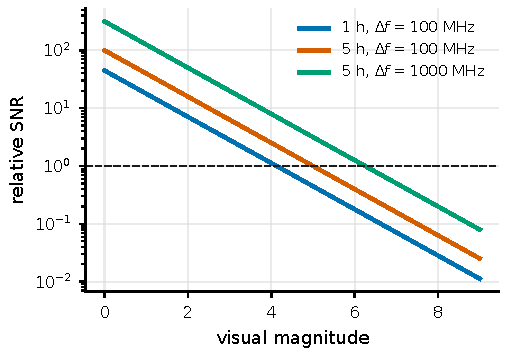
\includegraphics[width=0.86\linewidth]{figures/generated/chapter_05/ch05_snr_scaling.pdf}
\caption{The relative scaling of the intensity-interferometry SNR. For each magnitude a star is fainter, the photon spectral flux drops to about \(0.398\) of its original, and the SNR falls linearly in proportion; whereas integration time and electronic bandwidth improve the SNR only as the square root: quadruple the exposure for double the SNR. The curves omit collecting area, efficiency, background dilution, and \(|V|^2\), precisely to highlight: bright-star selection and high-speed electronics (linear factors) are far more worthwhile than "toughing out a few more nights" (the square-root factor).}
\label{fig:e11-snr-scaling}
\end{figure}

\paragraph{Substituting Real Numbers: the Order of Magnitude of Le Bohec--Holder}
\label{sec:e11-snr-lebohec}

An abstract formula must be brought down to earth by substituting real parameters. Le~Bohec and Holder, in assessing the feasibility of using Cherenkov arrays for intensity interferometry, made a classic estimate \citep{2006ApJ...649..399L}: taking two \(A=100\,{\rm m^2}\) telescopes, detection efficiency \(\alpha=0.3\), electronic bandwidth \(\Delta f=1\,{\rm GHz}\), and integration time \(T=5\,{\rm hr}\), at a baseline where the squared visibility \(|\gamma_{12}|^2=0.5\), one can measure a star of about \(V=6.7\) magnitude at \(5\sigma\) significance; for a brighter \(V=5\) magnitude star, the angular-diameter precision can reach a few percent. Compare this with the two conclusions of the last section: this \(V=6.7\) limiting sensitivity is held up almost entirely by those few linear factors (large area, high efficiency, GHz bandwidth); to push a magnitude fainter, one relies not on adding time (the square root, too expensive) but on continuing to add area and efficiency.

Set it against historical instruments, and the order of magnitude comes alive at once. Narrabri used two \(6.5\,{\rm m}\)-diameter light collectors, a \(443\,{\rm nm}\) central wavelength, a \(10\,{\rm nm}\) filter, a photocathode quantum efficiency of about 25\%, and an effective electronic bandwidth of only about \(60\,{\rm MHz}\) \citep{1967MNRAS.137..375H,1974MNRAS.167..121H,1974iiia.book.....H}. Substituting these numbers into Eq.~\eqref{eq:e11-snr} makes clear why its sample could be limited only to the very brightest stars (apparent magnitude roughly \(B<2.5\)): with area smaller than modern and bandwidth more than an order of magnitude smaller, several linear and square-root factors stacked together pin the sensitivity firmly on bright stars. VERITAS, meanwhile, uses four \(12\,{\rm m}\) telescopes, 250 MS/s sampling plus offline correlation, and can measure stellar diameters within a few hours even during the near-full-moon "dead time" unusable for gamma-ray observation \citep{2020NatAs...4.1164A}: this is exactly the result of those few linear factors (area \(\times3.4\), improved efficiency) joining forces with a wider electronic bandwidth.

\section{How to Judge Whether an Observation Is Real Signal or the Instrument Playing Tricks}
\label{sec:e11-feasibility}

The SNR formula tells you "bright enough, long enough," but it assumes the noise is clean white noise. In real observations the deadliest enemy is not white noise, but two kinds of things that masquerade as signal: \emph{background light} and \emph{systematic correlation}. Because the true signal itself is only one part in a million to one part in a thousand, any unmasked systematic effect can lead the angular-diameter fit into a ditch.

\paragraph{Background Harms in Two Ways at Once}
\label{sec:e11-background}

Moonlight, night-sky background, neighboring starlight mixed into a broadened point-spread function (PSF), detector dark current: these non-target photons are collectively called background. They harm the observation in \emph{two ways, acting simultaneously}:

\textbf{First, increasing shot noise.} Background photons must also be detected and must also take part in the coincidence count, and the shot noise they contribute directly raises the noise floor in the denominator of Eq.~\eqref{eq:e11-snr}, dragging the SNR down.

\textbf{Second, multiplying by an \(f_1f_2\) dilution factor.} Look back at Eq.~\eqref{eq:e11-correlation-model}: the correlation peak is multiplied by \(f_1f_2\), the product of the fractions of target photons out of the total photons in the two telescopes. This one is more insidious, because it is \emph{multiplicative}. Take a number: if target photons make up only 70\% in each telescope (\(f_1=f_2=0.7\)), the correlation amplitude is suppressed to
\[
  f_1 f_2 = 0.7\times0.7 = 0.49,
\]
leaving less than half. To recover the same significance from this half-strength signal, by the square-root scaling of the SNR, the integration time must be increased to about 4 times, and the longer the integration, the more likely various slow systematic drifts are to surface. Le~Bohec and Holder pointed out long ago that a Cherenkov telescope's wide optical PSF, of order \(0.05^\circ\), makes the night sky the boundary on faint-star sensitivity; modern VERITAS analysis too must specifically correct for night-sky background and dark current, or the angular diameter can be pulled off by about 10\% \citep{2006ApJ...649..399L,2020NatAs...4.1164A,2025ApJ...995..191A}. This is why narrowband filters and small-field stops are so important in intensity interferometry: they do not boost the signal, but they are the key to pushing \(f_1,f_2\) up toward 1.

\begin{figure}[tbp]
\centering
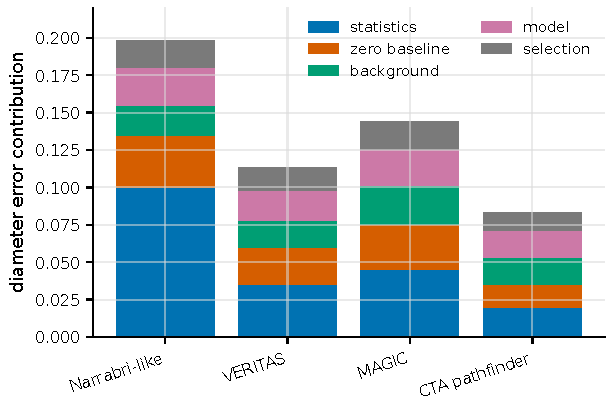
\includegraphics[width=0.82\linewidth]{figures/generated/chapter_05/ch05_error_budget.pdf}
\caption{The composition of the angular-diameter error budget in intensity interferometry. Statistical error (photon noise) falls as the square root of photon number and integration time, but zero-baseline calibration, background dilution, the stellar-atmosphere model, and weather/selection functions together build a floor of systematic error. Whether modern arrays can produce scientific results depends on whether these systematic terms, together with photon noise, can be honestly written into the likelihood function, rather than "toughed out" by the square root of time.}
\label{fig:e11-error-budget}
\end{figure}

\paragraph{Systematic Correlation Is More Dangerous Than White Noise}
\label{sec:e11-systematics}

White noise is at least "fair": it is random and can be pressed down by averaging. What truly keeps one awake is \textbf{systematic correlation}: some \emph{non-celestial}, yet synchronous, thing in the two signals. Ground reflection, a shared clock, power-supply ripple, temperature coupling, fiber crosstalk: all can inject a false correlation peak into the two electrical signals. It is more dangerous than white noise precisely because the true signal is only \(10^{-6}\) to \(10^{-3}\): however large the white noise, it tends to zero after averaging; but a systematic correlation of even \(10^{-5}\) will not be averaged away: it will sit there steadily, masquerading as a "visibility."

There is no single trick against it, only a whole set of cross-checks. The following are standard maneuvers in intensity-interferometry analysis, worth memorizing as a checklist:

\begin{itemize}
  \item \textbf{It must be zero far from zero delay.} The true thermal-light bunching peak appears only where the two signals are \emph{time-aligned}; pull the relative delay far from zero, and the correlation should return to zero. If there is a residual there, systematic correlation is at work.
  \item \textbf{The peak should vanish after swapping channels or an artificial time shift.} Swap the two signals, or deliberately insert an unphysical time offset, and the true signal peak will move or vanish with it; if the peak does not budge, it did not come from the sky.
  \item \textbf{The zero-baseline response \(N_0\) must be consistent everywhere.} Measure the same "zero-baseline" bunching height with different telescope pairs, different nights, different moon distances, and different electronic chains, and the \(N_0\) obtained should agree with one another. Once \(N_0\) shifts systematically, the \(|V|^2\) of all baselines in Eq.~\eqref{eq:e11-correlation-model} is stretched as a whole, and angular diameter, limb darkening, and oblateness all go wrong with it.
  \item \textbf{\(|V|^2\) should vary with \emph{baseline}, not with current.} The visibility of the same target should be a function only of the projected baseline \(B\); if instead it drifts along with the PMT anode current, ambient temperature, or electronic gain, then what drifts is the instrument, not the star.
\end{itemize}

MAGIC's intensity-interferometry system (MAGIC-SII) is a good example of engineering this discipline: it reuses the regular camera pixels, adds narrowband filters, transmits the signal out via VCSEL analog fiber, aggregates an electronic bandwidth of about \(110\,{\rm MHz}\), and uses a GPU real-time deadtime-free correlator to correlate online, ultimately reporting the diameters of 22 stars \citep{2024MNRAS.529.4387A}. It has pushed the limitation from "telescope area" toward "engineering stability and the calibration system," confirming exactly this: when the signal is as shallow as one part in a million, whether the systematic correlation can be held down often decides success or failure more than how large the mirror is.

\begin{figure}[tbp]
\centering
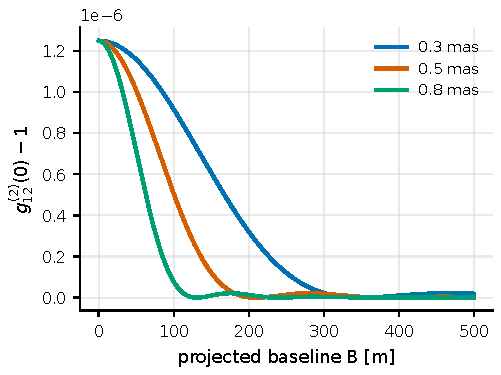
\includegraphics[width=0.86\linewidth]{figures/generated/chapter_05/ch05_sii_signal_vs_baseline.pdf}
\caption{The intensity-interferometry signal versus baseline, estimated with \(C_{12}=N_0|V|^2\) (\(N_0\) taken as \(1.25\times10^{-6}\), of the order of a modern blue-light system). The larger the star's angular diameter, the sooner \(|V|^2\) drops with baseline and shows a zero; hence the same set of baselines is more sensitive to a 0.8 mas star than to a 0.3 mas star. The first thing in observation design is to place the baselines, following the target's curve, in the "descending region," where there is both appreciable signal and maximal sensitivity to angular diameter.}
\label{fig:e11-sii-signal}
\end{figure}

\section{From Two to a Field: Multiple Baselines and uv Coverage}
\label{sec:e11-uv}

Two telescopes, however long they tough it out, can give you only a single \(|V|^2\) on \emph{one} projected baseline. And the previous chapter's van~Cittert--Zernike theorem tells us that the object's image is the inverse Fourier transform of its visibility over the whole \((u,v)\) plane. So to move from "a number" to "a picture," the only way out is to \emph{sample more spatial frequencies}. This section discusses how three things together spread the sampling from one point into a whole field.

\paragraph{More Telescopes, and the Baseline Count Explodes}
\label{sec:e11-baseline-count}

The first thing is the simplest: put out more telescopes. If the array has \(N\) telescopes, any two form a baseline, and the number of baselines that can be formed simultaneously is the combination "choose 2 from \(N\)":
\begin{equation}
  N_{\rm base}=\binom{N}{2}=\frac{N(N-1)}{2}.
  \label{eq:e11-baseline-number}
\end{equation}
\begin{formulaexplain}
\(N_{\rm base}\) is the number of telescope pairs (i.e.\ baselines) that can be formed simultaneously, and \(N\) is the number of telescopes. Each pair gives one independent baseline, so the baseline count grows explosively with array size, roughly as \(N^2/2\).
\end{formulaexplain}
The origin of the combination \(\binom{N}{2}\) is standard counting: the first telescope has \(N\) choices, the second the remaining \(N-1\), but "A-B" and "B-A" are the same baseline, so divide by 2. Substitute a few numbers to see how worthwhile it is: \(N=2\) has only 1 baseline; \(N=4\) (VERITAS) suddenly has 6; \(N=17\) has 136; and a CTAO-class few dozen to over a hundred telescopes can give thousands of baselines at once. The baseline count rising as \(N^2\) is the fundamental advantage of array telescopes over a two-antenna setup.

Here we must point out a sweet spot \emph{unique} to intensity interferometry. Amplitude interferometry (amplitude interferometry) must split the same coherent light beam optically among several beam combiners, and each split loses a share of photons, so with more paths the signal thins out. Intensity interferometry does not combine beams in optics; it first detects each telescope's light into an \emph{electrical signal}, and an electrical signal can be \textbf{losslessly copied} into arbitrarily many correlators. So one telescope's signal can be correlated with every other one at once, capturing all \(N(N-1)/2\) baselines in one go, with no "splitting light" between telescopes at all. For imaging that pursues dense \((u,v)\) coverage, this is intensity interferometry's natural bargain.

\paragraph{Let the Earth Turn for You: One Baseline Sweeps Out a Track}
\label{sec:e11-earth-rotation}

The second thing costs nothing: wait for the Earth to rotate. A telescope pair's separation vector on the ground is fixed, but its component \emph{projected onto the sky plane perpendicular to the line of sight} changes continuously as the target rises and sets in the sky. Recall the previous chapter's definition: the spatial frequency is the projected baseline divided by the wavelength, \(u=B_x/\lambda,\ v=B_y/\lambda\). As the Earth turns the target from east to west, the projected baseline \((B_x,B_y)\) varies continuously, so the same fixed telescope pair, over one night, has its sampling point \emph{draw out an arc across the \((u,v)\) plane}. This "Earth-rotation synthesis" is a decades-old stock-in-trade of radio interferometry, and it applies just as well to intensity interferometry: as long as the correlation result is stored every few minutes, one sampling point is stretched into a track.

\paragraph{Multiple Nights, Multiple Hour Angles, Multiple Telescope Pairs: Piecing Out Two-Dimensional Coverage}
\label{sec:e11-2d-coverage}

The third thing is to superpose the first two repeatedly. In one night the Earth can turn through only a segment of hour angle, drawing a finite arc; but change nights, change seasons, and observe the target at various hour angles, and the arcs join segment by segment. Then superpose the tracks of \emph{every} telescope pair in the array onto the same \((u,v)\) plot: each pair draws one, plus its conjugate point symmetric about the origin (because the real brightness distribution guarantees \(V(-u,-v)=V^*(u,v)\), so the negative-frequency point is equally a constraint), and finally, from a scattering of a few points, a two-dimensional \((u,v)\) coverage is pieced out. The denser the coverage, the finer the celestial structure that can be distinguished: sparse sampling suffices only to fit a diameter, and only dense sampling can distinguish disks, ellipses, binary stars, and even surface bright spots \citep{2008AIPC..984..205L,2012MNRAS.419..172N,2013APh....43..331D}.

\begin{figure}[tbp]
\centering
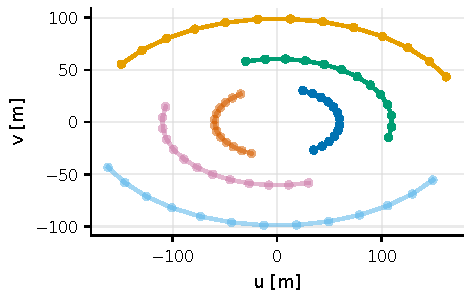
\includegraphics[width=0.82\linewidth]{figures/generated/chapter_05/ch05_uv_coverage.pdf}
\caption{A fixed telescope baseline is projected to different \((u,v)\) positions as the Earth rotates. Each colored track represents the spatial frequencies one telescope pair sweeps through over a night's hour-angle change, and the conjugate points symmetric about the origin (on the dashed side) are also effective Fourier constraints on the real brightness distribution. Superposing multiple pairs, multiple nights, and multiple hour angles grows the sampling from isolated points into two-dimensional coverage: the denser the coverage, the better one can distinguish disks, ellipses, binaries, and surface spots.}
\label{fig:e11-uv-coverage}
\end{figure}

\section{What to Do When the Phase Is Lost: Closure Phase, Phase Retrieval, and Low-Dimensional Models}
\label{sec:e11-phase}

Here we must face the innate weak spot of intensity interferometry. Amplitude interferometry directly measures the complex visibility \(V=|V|e^{i\phi}\), obtaining modulus and phase together; intensity interferometry measures only \emph{the degree of synchrony of the intensity fluctuations}, obtaining \(|V|^2\): \textbf{the phase \(\phi\) is lost}. This is no small matter: the Fourier phase encodes exactly "which way the brightness leans." The most immediate consequence of losing the phase is a kind of mirror degeneracy: a brightness distribution \(I(l,m)\) and its central-inversion mirror \(I(-l,-m)\) have \emph{exactly the same} \(|V|^2\), and the squared visibility alone can never separate the two. Measuring only the squared modulus amounts to knowing only "how much fluctuation there is" at each spatial frequency, without knowing "where the phase of the fluctuation is aligned." To reconstruct a true image, one must find a way to recover the phase information. There are three routes.

\paragraph{Route One: Third-Order Closure Phase}
\label{sec:e11-closure}

The first route inherits the third-order coherence function \(g^{(3)}\) of Chapter \ref{chap:e08}. When that third-order formula lands on three telescopes \(1,2,3\), a term appears:
\begin{equation}
  2\,{\rm Re}\big(\gamma_{12}\,\gamma_{23}\,\gamma_{31}\big),
  \label{eq:e11-triple}
\end{equation}
\begin{formulaexplain}
\(\gamma_{12},\gamma_{23},\gamma_{31}\) are the complex degrees of coherence on the three edges. Their product adds the phases of the three edges together: \(\phi_{12}+\phi_{23}+\phi_{31}\). This phase sum "once around the triangle" is the closure phase.
\end{formulaexplain}
The key lies in the phase of this triple product. Suppose each telescope introduces an unknown "piston" phase \(\psi_i\) from the atmosphere or instrument; it adds \(\psi_j-\psi_i\) to the phase of each edge. Add the three edges once around the triangle:
\[
  (\psi_2-\psi_1)+(\psi_3-\psi_2)+(\psi_1-\psi_3)=0.
\]
That annoying unknown phase of each telescope \emph{cancels exactly}! The remaining phase sum \(\phi_{12}+\phi_{23}+\phi_{31}\) belongs only to the celestial object itself, and this quantity is called the \textbf{closure phase}. It is conceptually exactly the old weapon against atmospheric jitter in amplitude interferometry, now reappearing in intensity interferometry in the guise of third-order correlation, and naturally immune to any single telescope's phase drift.

There is no free lunch: the third-order signal is much weaker than the second. The second order relies on the correlation of photons arriving \emph{in pairs}, while the third requires photons to arrive \emph{three at a time} together, and triplets are far rarer than pairs, with harsher error propagation. So the closure phase suits very large arrays and extremely bright targets, rather than being the default product of every observation.

\paragraph{Route Two: Two-Dimensional Coverage + Phase-Retrieval Algorithm + Physical Priors}
\label{sec:e11-phase-retrieval}

The second route bypasses phase measurement and \emph{solves back} the phase directly from a dense two-dimensional \(|V|\) distribution. This sounds like conjuring something from nothing, but mathematically it is not hopeless: for a real brightness distribution of compact support, its Fourier modulus and phase are not entirely independent, and the analytic structure of the modulus (via the Cauchy--Riemann relations) imposes constraints on the phase. Gerchberg--Saxton iteration \citep{1966JOSA...56..441G} and regularized reconstruction algorithms like MIRA project back and forth between the two constraints "match the measured \(|V|\)" and "satisfy the physical priors," forcing out a self-consistent phase. Here the \textbf{physical priors} are the crux: brightness non-negative, source of finite size, brightness distribution smooth, and, where necessary, a stellar-atmosphere template imposed: it is precisely these priors that filter out the mirror degeneracy and the infinitely many spurious solutions. Nuñez et al.'s simulations show that, under CTA-class \((u,v)\) coverage, bright thermal stars, fast rotators, binaries, and stars with surface spots can all be recovered to physically meaningful shape parameters, but success depends on the SNR, whether the short-baseline coverage is sufficient, and how the prior mask and image regularization are set \citep{2012MNRAS.419..172N,2012MNRAS.424.1006N,2014SPIE.9146E..0ZD}.

\paragraph{Route Three: Simply Don't Reconstruct the Image, Use a Low-Dimensional Model}
\label{sec:e11-low-dim}

The third route is the most pragmatic, and often the most powerful: \emph{do no model-free image reconstruction at all}, but take a physical model with only a few parameters and fit \(|V|^2\). Do not forget: measuring only \(|V|^2\) by no means limits one to measuring the diameter. For a large class of low-dimensional models (uniform disk, elliptical disk, binary star, limb darkening), the squared visibility can already give \emph{very strong} constraints. The visibility of a uniform disk is \(V(B)=2J_1(x)/x\) (\(x=\pi\theta B/\lambda\), with the angular diameter set in Chapter \ref{chap:e10} by the Bessel function's first zero \(x=3.8317\)); a flattened ellipse makes the zero-baseline vary with azimuth, a binary superposes a layer of cosine oscillation on \(|V|^2\), and limb darkening slightly reshapes the first lobe. All these differences can be read off from the \(|V|^2\) curve \emph{without needing the phase}. When the scientific goal is "how big is this star, how flattened, is it a binary" rather than "give me a model-independent photograph," a few-parameter model is often more stable and more credible than laborious phase retrieval.

\section{Why an Old Method Comes Back to Life: From Narrabri to CTAO}
\label{sec:e11-history}

String together all the preceding tools, and one can understand the tortuous technical history of intensity interferometry: it was once sentenced to death, and came back to life, unchanged, half a century later.

\textbf{Narrabri (1960s--1970s): proving the route works.} Australia's Narrabri Stellar Intensity Interferometer was the first instrument to fully demonstrate the scientific capability of this method. Two \(6.5\,{\rm m}\)-diameter light collectors worked on a variable rail baseline of 10--188 m, with a filter centered at about \(443\,{\rm nm}\) and bandwidth \(10\,{\rm nm}\), a photocathode quantum efficiency of about 25\%, and an effective electronic bandwidth of about \(60\,{\rm MHz}\). It measured the angular diameters of 32 stars and several binaries, the smallest diameter about \(0.4\,{\rm mas}\) \citep{1967MNRAS.137..375H,1967MNRAS.137..393H,1974MNRAS.167..121H,1974iiia.book.....H}. But it was subsequently retired, for exactly the reason that those few linear factors in Eq.~\eqref{eq:e11-snr} could not be raised at the time: movable large-area light collectors were expensive, low-noise high-speed electronics were immature, and multi-baseline imaging capability was lacking. The old method was not wrong; it was that the hardware of the time was unworthy of it.

\textbf{VERITAS (2019--): an old idea meets ready-made large mirrors.} The turning point came from atmospheric Cherenkov telescope arrays. Built originally to catch the nanosecond Cherenkov flashes triggered by gamma rays, they naturally have 10-m-class apertures, large-area mirrors, fast PMTs, long baselines, and acceptable optical image quality, exactly everything intensity interferometry had once yearned for. VERITAS uses four \(12\,{\rm m}\) telescopes to form 6 baselines at once, and measured uniform-disk diameters of \(\theta_{\rm UD}=0.523\pm0.017\,{\rm mas}\) and \(0.631\pm0.017\,{\rm mas}\) for \(\beta\)~CMa and \(\epsilon\)~Ori, at better than 5\% precision, in only a few hours, and "on the side" during near-full-moon periods unusable for gamma-ray observation \citep{2020NatAs...4.1164A}. As the \((u,v)\) coverage improved, its follow-up observations of \(\beta\)~UMa and the fast rotator \(\gamma\)~Cas advanced from "measuring a radius" to "measuring a direction-dependent shape": \(\gamma\)~Cas, using 6 baselines and over 160 pair-hours of data, yielded the oblateness of the optical photosphere, with a minor-axis diameter of about \(0.43\,{\rm mas}\), a major-to-minor axis ratio of about 1.28, and a rotation-axis position angle of about \(116^\circ\) \citep{2024ApJ...966...28A,2025ApJ...995..191A}.

\textbf{MAGIC-SII (2024): turning it into a switchable standard mode.} MAGIC uses two \(17\,{\rm m}\) parabolic telescopes, reusing the existing camera pixels, with VCSEL analog-fiber transmission and a GPU real-time deadtime-free correlator (aggregate bandwidth about \(110\,{\rm MHz}\)), achieving fast switching between regular gamma-ray observation and intensity-interferometry mode, and reported the diameters of 22 stars \citep{2024MNRAS.529.4387A}. What it demonstrates is not merely "it can measure," but "it can run stably as the routine side job of a mature facility."

\textbf{CTAO (under construction): toward kilometer baselines and thousands of baselines.} The next-generation CTAO pulls both of intensity interferometry's great levers to the full. Kilometer-scale baselines at 350--450 nm correspond to \emph{tens of microarcseconds} of resolution, one or two orders finer than Narrabri; and by Eq.~\eqref{eq:e11-baseline-number}, a few dozen to over a hundred telescopes can give \emph{thousands} of baselines and extremely dense \((u,v)\) coverage, which is exactly the prerequisite on which the phase retrieval and image reconstruction of Section \ref{sec:e11-phase} rely. It will not replace amplitude interferometers like CHARA and VLTI (which have their own strengths in sensitivity, phase capability, and the infrared band) but will become a complementary sharp tool: specializing in blue light, ultra-long baselines, bright hot stars, and fast-varying objects \citep{2013APh....43..331D,2014SPIE.9146E..0ZD}.

To close this history in one sentence: the old method came back to life not because the idea changed, but because those few linear factors in Eq.~\eqref{eq:e11-snr} (area, efficiency, bandwidth, baseline count) were finally fed to satiety all at once by Cherenkov arrays. The physics had always been there waiting; it was the hardware that arrived late.

\section{Chapter Summary}
\label{sec:e11-summary}

\begin{itemize}
  \item \textbf{The SNR formula is the first abacus.} \((S/N)_{\rm rms}=A\,\alpha\,n\,|\gamma_{12}|^2(\Delta f\,T/2)^{1/2}\): that square root comes from "averaging over \(M\sim\Delta f\,T\) independent samples, the noise shrinking as \(1/\sqrt{M}\)" (Chapter \ref{chap:e03}).
  \item \textbf{Two conclusions to memorize.} The SNR is \emph{linearly} proportional to photon spectral flux, area, and efficiency (bright stars, large mirrors are key); but grows only as \((\Delta f\,T)^{1/2}\) (quadruple the exposure for double the SNR). Improvement relies on the linear factors, not on toughing out a few more nights.
  \item \textbf{Background harms two ways.} It both increases shot noise and multiplies the correlation amplitude by \(f_1f_2\) (a 70\% target fraction leaves only 0.49). Narrowband filters and small-field stops are the key to pushing \(f_1,f_2\) up toward 1.
  \item \textbf{Systematic correlation is more dangerous than white noise,} because the true signal is only \(10^{-6}\)--\(10^{-3}\). Standard checks: the correlation should be zero far from zero delay; the peak should vanish after swapping channels/an artificial time shift; \(N_0\) must be consistent everywhere; \(|V|^2\) should vary with baseline, not with current.
  \item \textbf{Multiple baselines lead to imaging.} \(N\) telescopes give \(N(N-1)/2\) baselines; Earth rotation lets each pair's baseline sweep out a \((u,v)\) track; multiple nights and hour angles piece out two-dimensional coverage. Intensity interferometry's unique bargain: the electrical signal can be losslessly copied to many correlators, with no need to split light between telescopes.
  \item \textbf{The phase problem has three routes.} Third-order closure phase (inheriting \(g^{(3)}\) of Chapter \ref{chap:e08}, piston cancels automatically, but the signal is weak); two-dimensional coverage + phase-retrieval algorithm + physical priors; and the most pragmatic, using low-dimensional models like uniform disk / elliptical disk / binary / limb darkening, \(|V|^2\) already strongly constraining the shape.
  \item \textbf{The quantitative reason the old method revived:} Narrabri (\(6.5\,{\rm m}\), 443~nm, \(\sim60\,{\rm MHz}\), 32 stars measured, smallest \(\sim0.4\,{\rm mas}\)) \(\to\) VERITAS (\(4\times12\,{\rm m}\), \(\beta\)~CMa/\(\epsilon\)~Ori precision <5\%) \(\to\) MAGIC-SII (\(2\times17\,{\rm m}\), GPU correlator, 22 stars) \(\to\) CTAO (kilometer baselines, tens of microarcseconds, thousands of baselines). The physics did not change; the hardware fed the linear factors of Eq.~\eqref{eq:e11-snr} to satiety.
\end{itemize}

\medskip
\noindent\textbf{Questions to Ponder.}
\begin{enumerate}
  \item One star is 2.5 magnitudes fainter than another, all else equal; to measure the same SNR, by roughly how many times must the integration time be lengthened? (Hint: first use the linear factor to find how many times the SNR drops, then convert to time via the square-root scaling.)
  \item How many baselines can an array of 6 telescopes form simultaneously? If 4 more are added to make 10, how many times the original is the baseline count? What does this mean for the \((u,v)\) coverage?
  \item Why can intensity interferometry tolerate very poor optical image quality, yet is extremely sensitive to the electronic time alignment? Contrast it with "amplitude interferometry requiring the optical path stable to a small fraction of a wavelength," and say where each of the two "precision budgets" is spent.
\end{enumerate}
